In this section we present the results derived from the measurements of the peak bolometric luminosity and the trends observed with other observables for the SNe in our low-reddening sample, as well as the complete sample of objects with a measured timing of the second maximum


\begin{table*}
\caption{$L_{max}$ measurements for low reddening SNIa with a measured $t_2$. }

\begin{center}
\begin{tabular}{llccccrrr}
\hline
SN  & $L_{max}(\cdot e^{43} erg s^{-1})$ & $e_{L}$  & $M_{Ni}-Arn (M_{\odot})$  & $M_{Ni}-Arn (M_{\odot})$ (fixed rise)  & $M_{Ni}-DDC (M_{\odot})$\\% & $E(B-V)_{MW}$ & u-band lum \\
\hline
%SN2001ba & 1.18 & 0.15 & 0.58 & 0.59 & 	0.57 \\
SN2002dj & 1.25 & 0.26 & 0.59 & 0.63 & 0.61 \\
SN2002fk & 1.42 & 0.23 & 0.68 & 0.71 & 0.76 \\
SN2005M & 1.37 & 0.08 & 0.70 & 0.69 & 0.71 \\
SN2005am & 1.1 & 0.2 & 0.47 & 0.55 & 0.52 \\
SN2005el & 0.91	& 0.11 & 0.40 & 0.46   & 0.44 	\\	
SN2005eq & 1.32 & 0.2 & 0.67 & 0.66 & 0.67 \\
SN2005hc & 1.36 & 0.2 & 0.69 & 0.68 & 0.71 \\
SN2005iq & 1.07 & 0.11 & 0.48 & 0.54 & 0.51 \\
SN2005ki & 1.03 & 0.27 & 0.45 & 0.51 & 0.49 \\
SN2006bh & 0.86 & 0.15 & 0.37 & 0.43 & 0.40 \\
SN2007bd & 1.22 & 0.13 & 0.55	  & 0.61 & 0.59	\\
SN2007on & 0.6 & 0.09 & 0.24 & 0.30 & 0.28 \\
SN2008R & 0.53 & 0.1 & 0.21 & 0.26 & 0.25 \\
SN2008bc & 1.24 & 0.19 & 0.60 & 0.62 & 0.63 \\
SN2008gp & 1.29 & 0.14 & 0.62 & 0.65 & 0.64 \\
SN2008hv & 1.08 & 0.13 & 0.48 & 0.54 & 0.52 \\
SN2008ia & 1.13 & 0.14 & 0.50 & 0.57 & 0.55 \\
SN2011fe & 1.1 & 0.15 & 0.50 & 0.55 & 0.52 \\
\hline
\end{tabular}
\label{tab:mni}
\end{center}
\end{table*}

\subsection{Correlation between $L_{max}$ and $t_2$ }

In figure ~\ref{fig:nit2}, we find that there is a very strong correlation between $t_2$ and $M_{Ni}$ in the $Y$ and $J$ bands with $r$ values of 
0.80, 0.88. A much weaker trend is observed in the $H$ band with $r \sim$ 0.60. This is reflected in the ratio of the slope to the slope error in equation \eqref{eq:lin_t2}

In the $Y$ and $J$ band, a strong correlation suggests that objects with more Ni produced show later second maxima. 

\begin{subequations}
\label{eq:lin_t2}
\begin{equation}
\label{eq:y}
L_{Max}=0.040(\pm 0.005) * t_2(Y) - 0.055 (\pm 0.125)
\end{equation}
\begin{equation}
\label{eq:j}
L_{Max}=0.042(\pm 0.004) * t_2(J) - 0.039 (\pm 0.102)
\end{equation}
\begin{equation}
\label{eq:j}
L_{Max}=0.033(\pm 0.009) * t_2(H) - 0.239 (\pm 0.203)
\end{equation}
\end{subequations}

The scatter around the best fit in $YJH$ bands is 0.18, 0.16 and 0.22 (* $e^{43} erg s ^{-1}$) respectively. This reflects the strength of the correlations in the individual bands

From the sample presented in Table \ref{tab:mni}, we reject objects with a total E(B-V) (host galaxy + MW) of $\geq$ 0.1. As a result, 7 objects with $E(B-V)_{host}<$0.1 but total E(B-V) $\geq$ are removed. We do not find a substantial decrease in the correlation coefficients in the $YJH$ bands. Since we know the reddening law in the MW, which allows us to correct for the absorption by dust,  we include these objects in our analysis to have as large a sample as possible.

\iffalse
Using equations \eqref{eq:lin_t2} we can derive a relation between the luminosity at peak and the $t_2$
\begin{subequations}
%\begin{equation}
\begin{multline}
\label{eq:ly}
L_{max}=\alpha*[(1.79 (\pm 0.32) X 10^{42} e^{-t_R/8.8}  \\ + 4.04 (\pm 0.7) X 10^{41} e^{-t_R/111.3})* t_2(Y) \\ 
 - (1.41 (\pm 0.73) X 10^{43} e^{-t_R/8.8} + 3.06 (\pm 1.66) X 10^{42} e^{-t_R/111.3})]
\end{multline}
%\end{equation}
%\begin{equation}
\begin{multline}
\label{eq:lj}
L_{max}=\alpha*[(1.73 (\pm 0.26) X 10^{42} e^{-t_R/8.8}  \\ + 3.93 (\pm 0.55) X 10^{41} e^{-t_R/111.3})* t_2(J) \\
- (1.32 (\pm 0.66) X 10^{43} e^{-t_R/8.8} + 3.01 (\pm 1.43) X 10^{42} e^{-t_R/111.3})]
\end{multline}
\begin{multline}
\label{eq:lh}
L_{max}=\alpha*[(1.03 (\pm 0.48) X 10^{42} e^{-t_R/8.8} \\ + 2.31 (\pm 1.04) X 10^{41} e^{-t_R/111.3})* t_2(H) \\
- (7.92 (\pm 9.65) X 10^{42} e^{-t_R/8.8} + 1.61 (\pm 2.31) X 10^{42} e^{-t_R/111.3})]
\end{multline}
%\end{equation}
\end{subequations}
\fi
Equations \eqref{eq:ly,eq:lj,eq:lh} relate the timing of the second maximum to the peak bolometric luminosity by combining equation \eqref{eq:eni} with equation \eqref{eq:y,eq:j,eq:h}. We can see that the relation is dependent on the rise time of the SN and the $\alpha$ parameter which encodes the deviation from Arnett's rule.

From the equations it is evident that the timing of the second maximum in $H$ doesn't provide stringent constraints on the bolometric peak luminosity.



\subsection{Test Case for SN2014J and SN2006X}
Using the correlations derived above, we want to estimate the Ni masses of heavily reddened SNae. The first test case is the nearby SN 2014J in M82 with an $E(B-V)_{host}$ of 1.3. 
Current attempts to use the bolometric light curve depend on the $A_V$ value used and vary by a factor of $\sim$ 2
 (0.37 $M_{\odot}$ if using $A_V$=1.7 mag from \citet{Margutti2014}, compared to 0.77 using a higher $A_V$ of 2.5 mag from \citet{Goobar2014}).  In our analyses the aim is to 
 estimate the $M_{Ni}$ independent of the extinction.

The proximity of SN2014J, has allowed for the first $\gamma$ ray Co line detection in an SNIa (Churazov+ 2014). the authors, using a line photon escape fraction from the models, 
deduce an Ni mass of 0.62  $\pm$ 0.13 $M_{\odot}$. This measurement is
 independent of the $A_V$ value used and is one method of obtaining $M_{Ni}$ for highly reddened objects. However, $\gamma$ ray detections aren't possible for farther away SN, for which we require a different estimation method. 

Using the best fit relation for the sample defined above , we obtain $M_{Ni}$ of 0.57 $\pm$ 0.21 $M_{\odot}$  for a $t_2$ of 28.37 $\pm$ 5.7 days. 
Thus, we find a very good correspondence between the values from the $\gamma$ rays and the NIR second maximum. This adds evidence to the argument that the NIR can be used for estimate $M_{Ni}$ for highly reddened SN,
even in more distant objects for which $\gamma$ ray Co line detections are not possible
This uncertainty in $M_{Ni}$ can be reduced with a more precise estimate of $t_2$. 

For SN2014J, we can get a precise measurement of the extinction from IR spectra at $\sim$ +300 days. This is again not possible for 
objects farther away. Thus, we apply this relation to a farther away, heavily extinguished object, SN2006X. 
The measured value for SN2006X of $t_2(J)$ is 28.19 with an error of 0.63  days. This results in an $M_{Ni}$ value of 0.57 $\pm$ 0.13 $M_{\odot}$. We can see that a smaller uncertainty in $t_2$ gives a more accurate measurement of 
$M_{Ni}$. We compare this value for SN2006X to that obtained using $t_2(Y)$ and obtain $M_{Ni}$ of 0.58 $\pm$ 0.17 $M_{\odot}$. We find both these values consistent with each other. The slightly higher error bar on
 the value from $t_2(Y)$ is due to a larger error on the 
intercept in the best fit relation for the $Y$ band. 
For both SN2014J and SN2006X, the $t_2(H)$ gives an $M_{Ni}$ of 0.50 $\pm$ 0.26 $M_{\odot}$ and 0.51 $\pm$ 0.23 $M_{\odot}$ respectively. We can see that a weaker correlation in the $H$ band leads to a slight offset in the $M_{Ni}$ estimate and 
a larger error bar on the measurement. Hence, we conclude that using the $H$ band to measure the $M_{Ni}$ is not feasible

The derived value of $M_{Ni}$ is consistent with the conclusion that SN2006X is a 'normal' SNIa \citep{Wang2007,Patat2007}. 
\begin{table*}



\begin{center}
\caption{$M_{Ni}$ estimates for 5 objects with high values of $E(B-V)_{host}$. We present constraints from the relation using only $t_2(J)$ as well as from both $t_2(Y)$ and $t_2(J)$. We can see a marked decrease in the error values when combined constraints are used}
\begin{tabular}{llcccrr}
\hline
SN & $t_2(J)$ & $M_{Ni}$ (inferred) & $\sigma$ & $\mu$ & $e_{\mu}$ & Method \\
\hline
SN1986G	& 16.40 ($\pm$ 1.4)	&	0.32 & 0.10	& 28.01 & 0.12 & $J$ band relation \\
-- & --	& 0.33	& 0.08	&--&--& combined fit \\
SN2005A	& 27.58 ($\pm$ 0.3)	& 0.57	&  0.13 & 34.51 & 0.11  & $J$ band relation \\
-- & -- &	0.57	& 0.11	&--&--& combined fit \\
SN2006X	& 28.19  ($\pm$ 0.5)	& 0.57 & 0.13 &	 30.91 & 0.08 & $J$ band relation \\
-- & -- &	0.58	& 0.11	&--&--& combined fit \\
SN2008fp & 31.03 ($\pm$ 0.3)	& 0.64	& 0.15 & 31.79 & 0.05 & $J$ band relation \\
-- 	- &-- & 0.64	& 0.13	&--&--& combined fit		\\
SN2014J	& 31.99 ($\pm$ 1.2)	& 0.66	& 0.15 &  27.64 & 0.10   & $J$ band relation\\
--	& -- & 0.66  & 0.13 &--&--& combined fit \\
\hline
\end{tabular}

\label{tab:red}

\end{center}




\end{table*}



We include three more objects in the highly reddened sample, namely, 1986G, 2005A and 2008fp. We calculate the $M_{Ni}$ for these objects in the same way as for SN2014J and SN2006X. We summarise our findings in Table ~\ref{tab:red}.
We can see that 1986G has a lower value of $M_{Ni}$ than the other objects in the sample. This is consistent with the observed optical decline rate and lower $B$ band luminosity of the SN. Since we find that $t_2$ in both $Y$ and $J$ bands correlates very strongly with the $M_{Ni}$, we use combined constraints from the relations to obtain an $M_{Ni}$ estimate. We can see from Table ~\ref{tab:red} that the error on the $M_{Ni}$ reduces when using combined constraints. For 2014J, it is 0.17 $M_{\odot}$ whereas for the others it is much lower at 0.07 $M_{\odot}$ 


Hence, we conclude that the NIR second maximum timing (in $Y$ and $J$) is a very good indicator of the amount of Nickel synthesised in the explosion, even for heavily reddened objects. 


\subsection{Deriving $M_{Ni}$ from $L_{max}$}
In the sections above, we have found a strong correlation between the peak bolometric luminosity ($L_{max}$) and $t_2$ in the $Y$ and $J$ bands. 
%From this correlation we have derived a value for the peak bolometric luminosity of a sample of 5 highly reddened supernovae, which we have summarised in Table ~\ref{tab:red}.

Since our final aim is to derive a value of the Nickel mass for objects which have a measured value of $t_2$, we present the different methods to derive $M_{Ni}$ from the peak bolometric luminosity.

\subsubsection{Arnett's rule with a variable rise time}
Arnett's rule states that the luminosity of the SN at peak is given by the instantaneous rate of energy deposition from radioactive decays inside the expanding ejecta. 
This is summarized in equation \eqref{eq:lm-eni}. 
\begin{equation}
L_{max}=\alpha E_{Ni} (t_R)
\end{equation}

Where $E_{Ni}$ is the input from $^{56}$Ni decay at maximum, $t_R$ is the rise time and $\alpha$ accounts for deviations from Arnett's Rule.

\begin{equation}
\label{eq:eni}0.040(\pm 0.005) * t_2(Y) - 0.055 (\pm 0.125)
E_{Ni} (1 M_{\odot})= 6.45  X  10^{43} e^{-t_R/8.8} + 1.45  X  10^{43} e^{-t_R/111.3}
\end{equation}

For estimates using different rise times, we follow the relation in \citet{G2011}
\begin{equation}
t_{R, B}=17.5 + 5(\Delta m_{15} - 1.1)
\end{equation}
and  
\begin{equation}
t_{R, Bol}=t_{R, B}+ (t_{max, bol} -t_{max, B})
\end{equation}
which implies 

\begin{multline}
L_{max}=\alpha * (6.45  X  10^{43} e^{-((17.5 + 5(\Delta m_{15} - 1.1)
+t_{max, bol} -t_{max, B}))/8.8} + \\ 1.45  X  10^{43} e^{-(17.5 + 5(\Delta m_{15} - 1.1)+t_{max, bol} -t_{max, B}))/111.3})*(M_{Ni}/M_{\odot})
\end{multline}

substituting the relation derived between $L_{max}$ and $t_2$ we get a relation between $t_2$ and $M_{Ni}$
\begin{subequations}
\begin{multline}
(M_{Ni}/M_{\odot})=(0.040(\pm 0.005) * t_2(Y) - 0.055 (\pm 0.125))/\\(\alpha * (6.45  X  10^{43} e^{-((17.5 + 5(\Delta m_{15} - 1.1)
+t_{max, bol} -t_{max, B}))/8.8} + \\ 1.45  X  10^{43} e^{-(17.5 + 5(\Delta m_{15} - 1.1)+t_{max, bol} -t_{max, B}))/111.3})
\end{multline}
\begin{multline}
(M_{Ni}/M_{\odot})=(0.042(\pm 0.004) * t_2(J) - 0.039 (\pm 0.102))/\\(\alpha * (6.45  X  10^{43} e^{-((17.5 + 5(\Delta m_{15} - 1.1)
+t_{max, bol} -t_{max, B}))/8.8} + \\ 1.45  X  10^{43} e^{-(17.5 + 5(\Delta m_{15} - 1.1)+t_{max, bol} -t_{max, B}))/111.3})
\end{multline}
\begin{multline}
(M_{Ni}/M_{\odot})=(0.033(\pm 0.009) * t_2(H) - 0.239 (\pm 0.203))/\\ (\alpha * (6.45  X  10^{43} e^{-((17.5 + 5(\Delta m_{15} - 1.1)
+t_{max, bol} -t_{max, B}))/8.8} + \\ 1.45  X  10^{43} e^{-(17.5 + 5(\Delta m_{15} - 1.1)+t_{max, bol} -t_{max, B}))/111.3})
\end{multline}
\end{subequations}

Since the $\Delta m_{15}$ values are related very strongly to $t_2$ in the different bands, using a variable rise time leads to a non-linear relation between $t_2$ and $M_{Ni}$  
\subsubsection{Arnett's rule with a fixed rise time}
For this method of deriving $M_{Ni}$ from $L_{max}$, we use a fixed rise time of 19 days, as in \citet{stritzinger2006}. Similar to their analysis, we propagate an uncertainty of $\pm$ 3 days 
\begin{equation}
\label{eq:arn}
L_{max}=(2.0 \pm 0.3) X 10^{43} (M_{Ni}/M_{\odot}) erg s^{-1}
\end{equation}

For deriving equation \eqref{eq:arn}, we use $\alpha$=1. 

\subsubsection{Interpolating using DDC models}
From these bolometric light curves, we derive $M_{Ni}$ values by interpolating the relation between  $L_{bol}(max)$ and $M_{Ni}$ from the DDC models of \citet{Blondin2013}
For objects without NIR coverage near maximum, we interpolate the values for the synthetic pseudo-bolometric light curves 
calculated only using the UBVRI filters. For SN2004gu and SN2007nq, which only has near maximum coverage in the $BVRI$ filters, we use the model value for only that set of filters. 

\subsection{Complete NIR Sample}
Since we have derived the relation between $L_{max}$ and $t_2$ and have presented the different ways to obtain the $M_{Ni}$ from the $L_{max}$, we can then use the distribution of $t_2$ for all objects, independent of reddening to obtain a distribution of $M_{Ni}$ using the relations derived

\begin{figure}
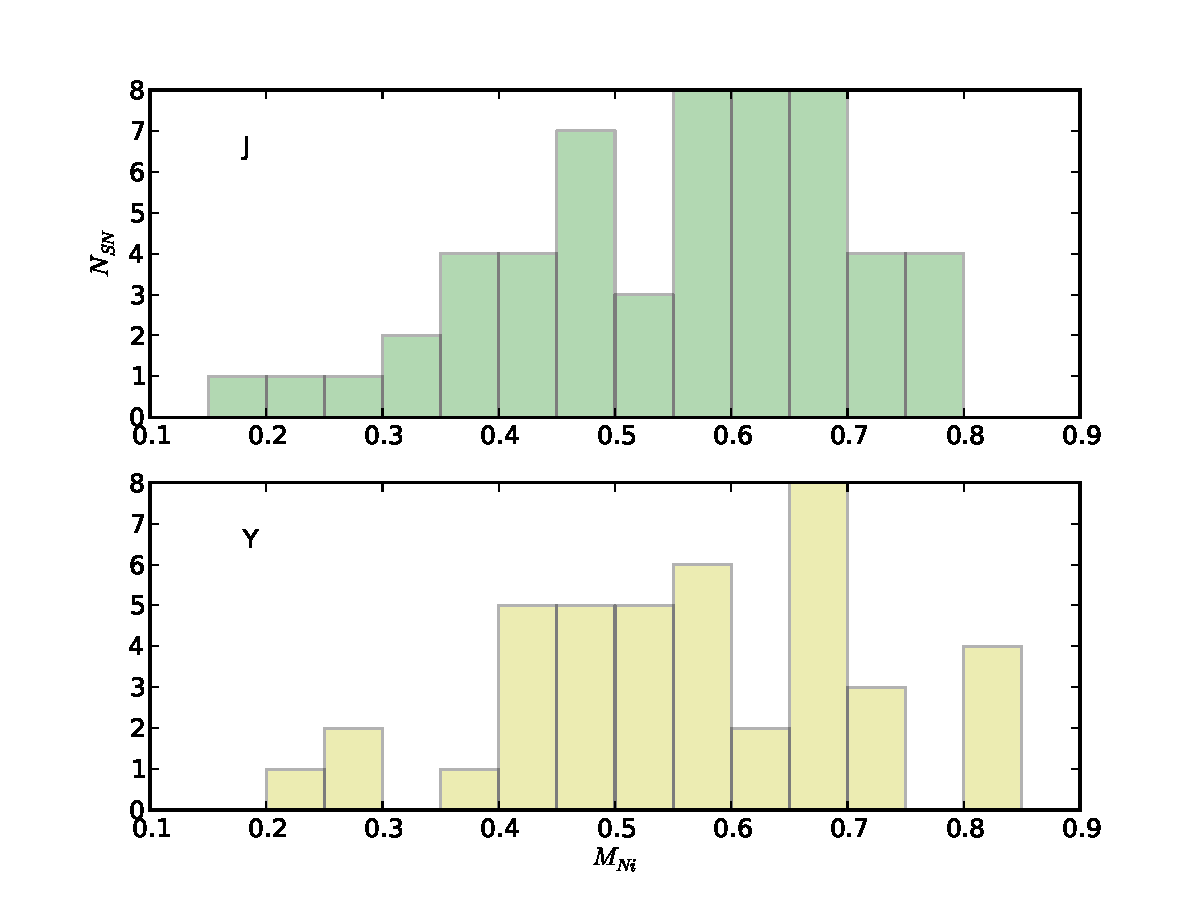
\includegraphics[width=.5\textwidth, trim= 0 30 0 30]{../plot_rel/nihist_rel.pdf}
\caption{Histogram distributions of $M_{Ni}$ derived from the distributions of $t_2$ for a complete sample of SNIa with measured $t_2$. This uses the Arnett's rule derivation with fixed }
\label{fig:hist}
\end{figure}

From figure \ref{fig:hist}, we find a large scatter in the $M_{Ni}$ values. We find that the objects vary by a factor of 3 in their $M_{Ni}$ distribution. We note, however, that since 91bg-like objects do not show a second maximum, we do not have values in the figure $\lesssim$ 0.2 $M_{\odot}$

\subsection{Comparison with published values}
We searched the literature for published values of $M_{Ni}$ for objects in our sample. In \citet{Scalzo2014} , the authors published values of $M_{Ni}$ for 2005el and 2011fe. For 2011fe, we find $M_{Ni}$ of 0.52 $\pm$ 0.15 $M_{\odot}$ whereas the value in S14 is 0.42 $\pm$ 0.08. We note that the value of $\alpha$ in their study is 1.2 whereas we use $\alpha$=1. Using their value of $\alpha$, we find $M_{Ni}$= 0.44 $M_{\odot}$, which is a better agreement. 

For SN2005el we find $M_{Ni}$ of 0.44 $\pm$ $M_{\odot}$. \citet{Scalzo2014} provides a discussion of this object, which in their sample they measure to have an $M_{Ni}$ of 0.52. It is one of two outliers in their $M_{Ni}$-$\Delta m_{15}$. They argue that it is likely for the SN to have a lower $M_{Ni}$ that their fiducial analysis suggests.  





\subsection{Bolometric Light Curve Shape}
Recent studies have shown that SNIa have remarkable uniformity in the late decline rate in NIR ($YJH$ bands). Studies like \citep{Barbon1973, Phillips1999, Leibundgut2000}
have shown that the late declines in the optical are very uniform as well, which indicates that the SNae have a similar structure of their ejecta. \citet{Contardo2000}
found a very late decline for the pseudo-bolometric light curves in their sample, with a mean decline rate of 2.6 mag per 100 days. We investigate the distribution of the exponential 
decline for objects in our sample.

We compute the decline rate of the pseudo-bolometric light curve between +40 and +90 days (measured with respect to $B_{max}$, however, we note that the value doesn't change significantly for phase
measured wrt. bolometric maximum). We find a very uniform distribution of $m$ for our objects, with $\overline{m}$=0.031 mag/day $\sigma$=0.0032. we note here that the decline rate calculated for our sample include YJH band late time data, which has been seen to have a signifcantly faster decline than the optical (0.05 mag/day compared to $\sim$ 0.01 mag/day in the optical). This explains why the average decline at late times is greater than the average for the C00 sample. 
For our objects we calculate the late decline in the BVRI pseudo-bolometric light curves to compare to the sample mean for C00. We find that $\overline{m}$ is 2.62 mag per 100 days with a scatter of 0.23 mag/day about the mean.   

This is consistent with the findings of \citet{Contardo2000}.
We look at the 91bg-likes with sufficient late time coverage in our sample and find that they have a slightly faster late decline rate and the scatter is higher than for normal Ia's. 


We investigate the near peak bolometric decline (parametrized as $\Delta m_{15}(bol)$) for our sample and find a small dispersion within the sample, similar to the findings of \citet{Contardo2000}.
The scatter for the complete sample is 0.18 mag for $\Delta m_{15}(bol)$, compared to the larger dispersion in $\Delta m_{15}$ from the SN(oo)Py fit of 0.30 mag. This is comparable to the dispersion found in the C00 sample.

\begin{figure}
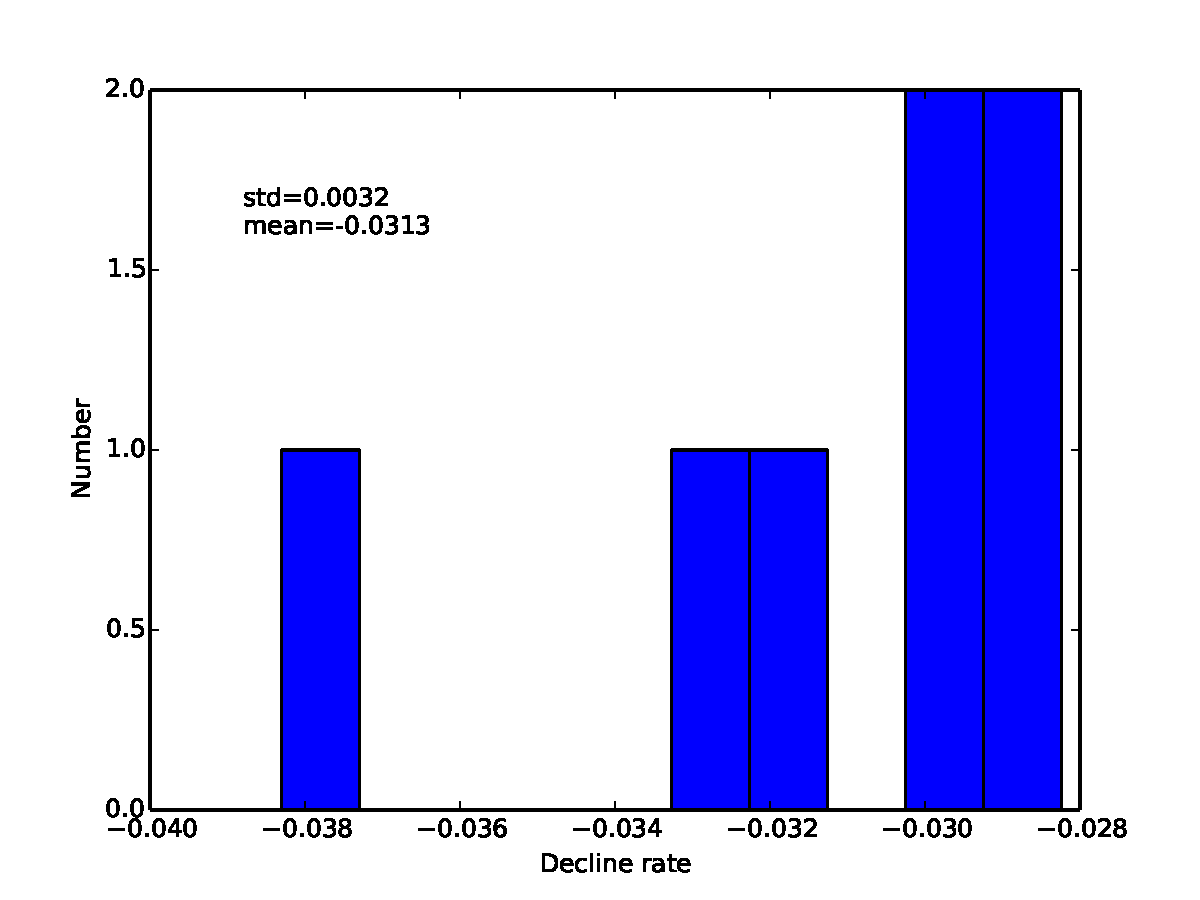
\includegraphics[width=0.5\textwidth, height=0.3\textwidth, trim=0 30 0 30]{../plot_rel/Late_decl_distrib.pdf}
\caption{The distribution of the late decline of the bolometric light curve (in magnitudes per day) for our sample of objects with sufficient coverage at late epochs (see text). We observe a very small
scatter in the sample}
\end{figure}
\begin{figure}
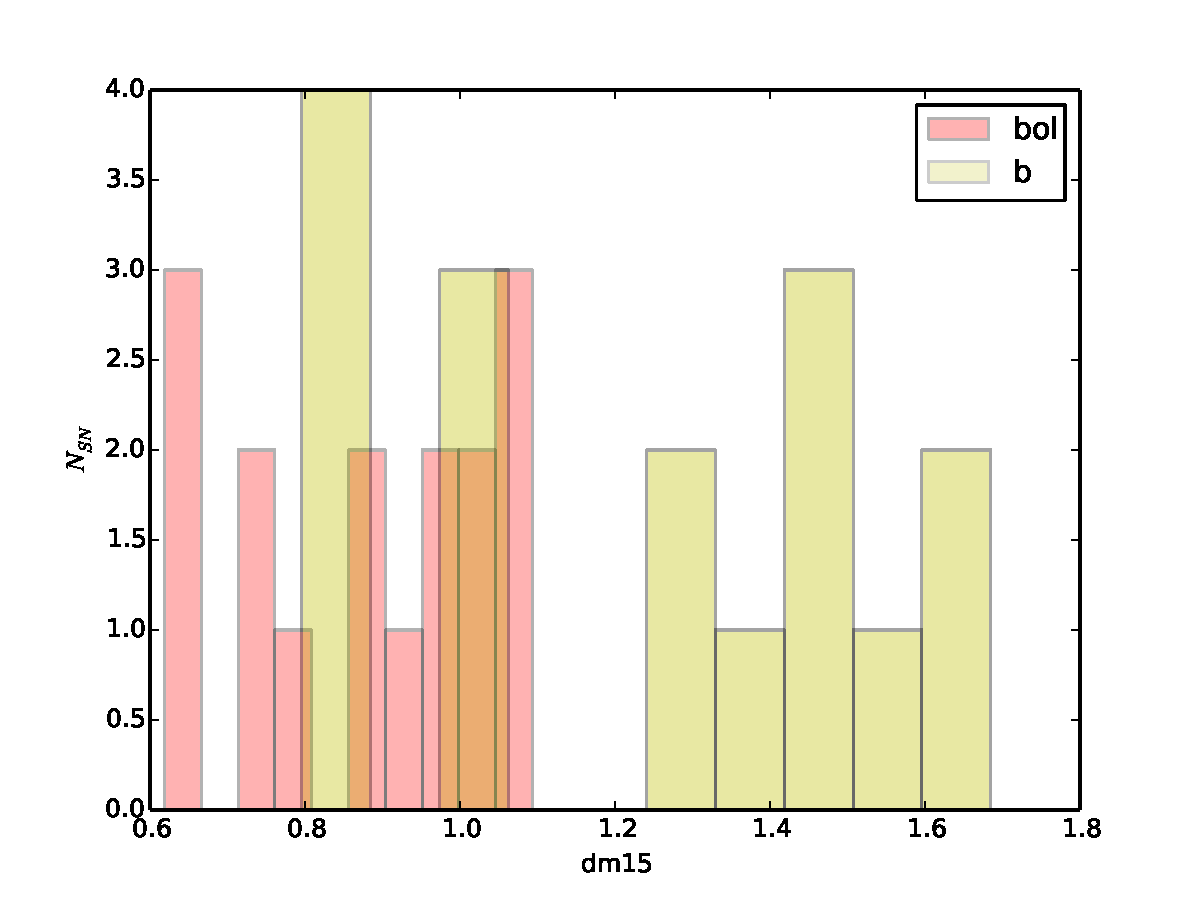
\includegraphics[width=0.5\textwidth, height=0.3\textwidth, trim=0 30 0 30]{../plot_rel/dm15_bol_b.pdf}
\caption{Comparison of the distribution of $\Delta m_{15}(bol)$ and  $\Delta m_{15}$ from SN(oo)Py. We find a narrower distribution of bolometric decline. We note that our sample doesn't
include objects in the $\Delta m_{15}$ range between 1.0 and 1.2 since none of these objects in the data pass the reddening cut}
\end{figure}
